\documentclass[t,aspectratio=169]{beamer} % 使用16:9宽高比
\usetheme{Madrid} % 选择Madrid主题
\usecolortheme{default} % 使用默认颜色主题

% 设置字体
\usepackage[UTF8]{ctex}
\usefonttheme{structurebold} % 加粗结构字体

% 数学包
\usepackage{amsmath, amssymb, bm}
\usepackage{url}

% 图形包 (如果需要插入图片)
\usepackage{graphicx}
% \graphicspath{{./images/}} % 假设图片放在images文件夹

% 标题页信息
\title[6.5.混合密度网络]{第6章：深度神经网络}
\subtitle{第5节：混合密度网络 (MDN)}
\author{《深度学习基础》课程小组}
% \institute{上海立信会计金融学院}
\date{\today}

\begin{document}

% 标题页
\frame{\titlepage}

% 目录页
\begin{frame}
    \frametitle{目录}
    \tableofcontents
\end{frame}

% 第一部分：引言
\section{引言}
\begin{frame}
    \frametitle{1. 引言：复杂条件分布的需求}
    \begin{itemize}
        \item 标准神经网络（NN）通常将 $ p(\mathbf{t} | \mathbf{x}) $ 建模为简单的分布（例如，回归任务中的高斯分布）。
        \item 这对于单峰、对称的分布效果很好。
        \item 然而，许多现实世界的问题涉及\alert{非高斯、多峰}的条件分布。
        \item 例如：逆问题（如机器人运动学）中，一个输入 $ \mathbf{x} $ 可能对应多个有效的输出 $ \mathbf{t} $。
        \item 解决方案：使用更灵活的分布族来建模 $ p(\mathbf{t} | \mathbf{x}) $。
    \end{itemize}
\end{frame}

% 第二部分：混合密度网络概念
\section{MDN的概念}
\begin{frame}
    \frametitle{2. 核心思想：混合密度网络 (MDN)}
    \begin{itemize}
        \item MDN 将标准神经网络与输出层的\alert{高斯混合模型 (GMM)} 相结合。
        \item 神经网络输出 GMM 的参数。
        \item 这使得网络能够表示复杂的、多峰的条件密度 $ p(\mathbf{t} | \mathbf{x}) $。
        \item 一般形式：
        \begin{equation*}
            p(\mathbf{t} | \mathbf{x}) = \sum_{k=1}^{K} \pi_k(\mathbf{x}) \, \mathcal{N}(\mathbf{t} | \boldsymbol{\mu}_k(\mathbf{x}), \sigma_k^2(\mathbf{x}) \mathbf{I})
        \end{equation*}
        \item 其中：
        \begin{itemize}
            \item $ K $: 混合分量的数量。
            \item $ \pi_k(\mathbf{x}) $: 分量 $ k $ 的混合系数（神经网络的输出）。
            \item $ \boldsymbol{\mu}_k(\mathbf{x}) $: 分量 $ k $ 的均值向量（神经网络的输出）。
            \item $ \sigma_k^2(\mathbf{x}) $: 分量 $ k $ 的方差（通常为各向同性，神经网络的输出）。
        \end{itemize}
    \end{itemize}
\end{frame}

% 第三部分：机器人运动学例子
\section{示例：机器人运动学}
\begin{frame}
    \frametitle{3. 示例：机器人臂逆运动学}
    \begin{itemize}
        \item 正向问题：给定关节角度 $ \theta_1, \theta_2 $，求末端执行器位置 $ (x, y) $。通常有唯一解。
        \item 逆向问题：给定末端执行器位置 $ (x, y) $，求关节角度 $ \theta_1, \theta_2 $。可能有多个解（例如，“肘部向上”vs“肘部向下”）。
        \item 预测 $ \mathbb{E}[\theta | x,y] $（均值）的标准神经网络会失败，因为两个有效解的均值可能是无效的。
        \item MDN 可以将 $ p(\theta | x,y) $ 建模为一个多峰分布，从而捕捉到这两个有效解。
    \end{itemize}
    % 如果有图，可以在此处插入
    \begin{figure}
        \centering
        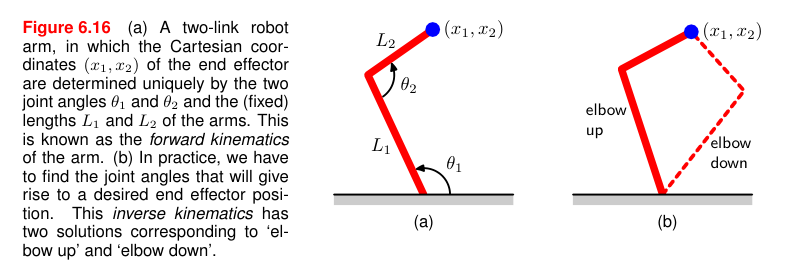
\includegraphics[width=0.5\textwidth]{fig616.png}
        \caption{机器人臂在相同末端位置下的两种可能构型。}
    \end{figure}
\end{frame}

% 第四部分：玩具例子
\begin{frame}
    \frametitle{4. 实验示例：逆函数}
    \begin{itemize}
        \item 考虑一个正向过程：$ x \rightarrow t = f(x) + \epsilon $ （带有噪声 $ \epsilon $）。
        \item 逆向问题是：给定 $ t $，推断 $ x $。这可能是高度多峰的。
        \item 生成数据：$ x_n \sim U(0,1) $，$ t_n = x_n + 0.3\sin(2\pi x_n) + \text{噪声} $。
        \item 交换角色：使用 $ t_n $ 作为输入，$ x_n $ 作为目标。
        \item 标准神经网络（最小二乘法）：对于多峰 $ p(x|t) $ 拟合效果差。
        \item MDN：能够捕捉 $ p(x|t) $ 的复杂形状。
    \end{itemize}
    % 如果有图，可以在此处插入
    \begin{figure}
        \centering
        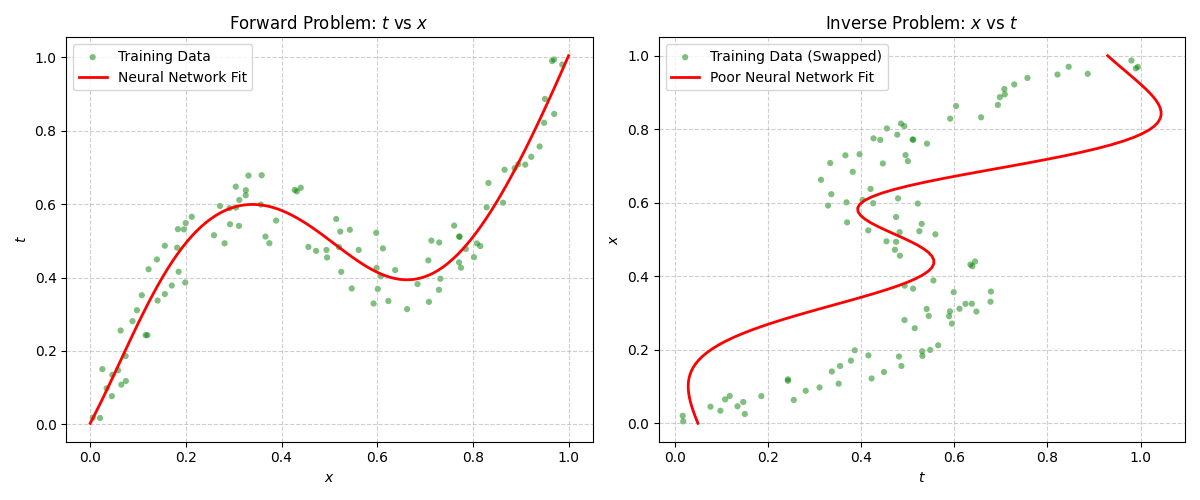
\includegraphics[width=0.4\textwidth]{fig617.png}
        \caption{左（正向问题）标准神经网络拟合效果好；右（逆向问题）拟合效果差。}
    \end{figure}
\end{frame}

% 第五部分：MDN架构
\section{MDN的架构}
\begin{frame}
    \frametitle{5. 混合密度网络的架构}
    \begin{itemize}
        \item 标准的前馈神经网络（例如，具有隐藏层的MLP）。
        \item 输出层有多个头（heads）：
        \begin{itemize}
            \item $ K $ 个单元用于混合系数 $ \pi_k(\mathbf{x}) $ （Softmax 激活函数）。
            \item $ K \times L $ 个单元用于均值 $ \mu_{k,j}(\mathbf{x}) $ （线性激活函数，其中 $ L $ 是 $ \mathbf{t} $ 的维度）。
            \item $ K $ 个单元用于方差 $ \sigma_k^2(\mathbf{x}) $ （Exp 激活函数以确保正值）。
        \end{itemize}
        \item 总输出数：$ K + K \times L + K = K(L+2) $。
        \item 神经网络学习将 $ \mathbf{x} $ 映射到参数 $ \{ \pi_k, \boldsymbol{\mu}_k, \sigma_k^2 \} $。
    \end{itemize}
    % 如果有图，可以在此处插入
    \begin{figure}
        \centering
        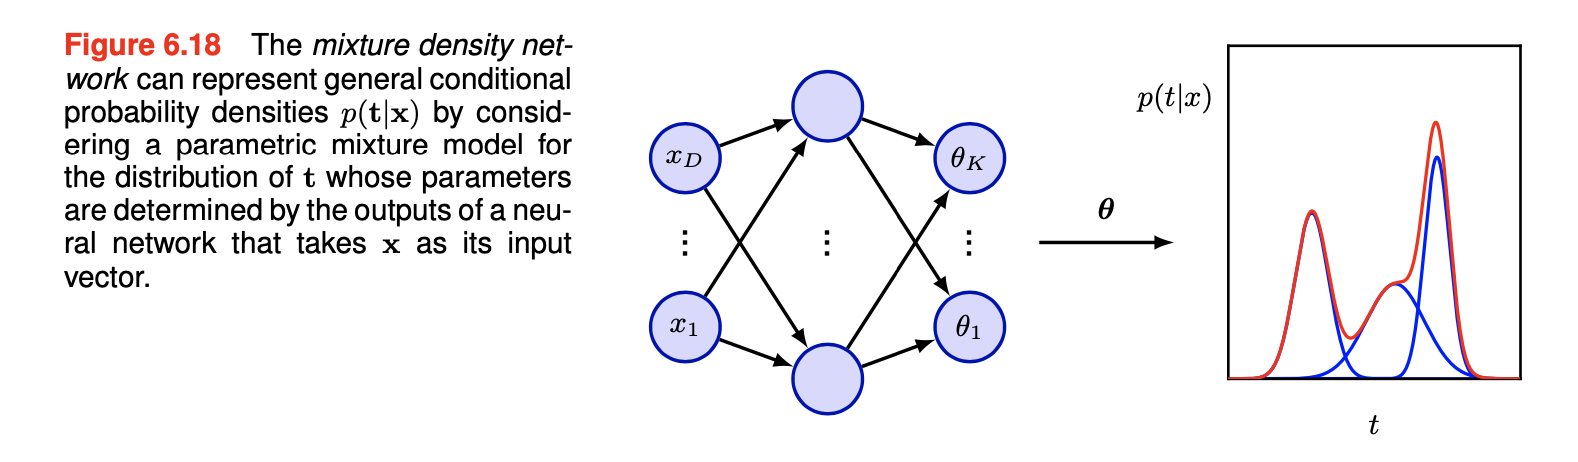
\includegraphics[width=0.6\textwidth]{fig618.png}
        \caption{混合密度网络的示意图。}
    \end{figure}
\end{frame}

% 第六部分：输出激活函数
\begin{frame}
    \frametitle{6. 输出激活函数}
    \begin{itemize}
        \item 混合系数 $ \pi_k(\mathbf{x}) $：
        \begin{itemize}
            \item 必须满足 $ \sum_k \pi_k = 1 $ 和 $ 0 \leq \pi_k \leq 1 $。
            \item 在预激活值 $ a_k^\pi $ 上使用 Softmax：
            \begin{equation*}
                \pi_k = \frac{\exp(a_k^\pi)}{\sum_{l=1}^{K} \exp(a_l^\pi)}
            \end{equation*}
        \end{itemize}
        \item 方差 $ \sigma_k^2(\mathbf{x}) $：
        \begin{itemize}
            \item 必须为正：$ \sigma_k^2 > 0 $。
            \item 在预激活值 $ a_k^\sigma $ 上使用指数函数：
            \begin{equation*}
                \sigma_k^2 = \exp(a_k^\sigma)
            \end{equation*}
        \end{itemize}
        \item 均值 $ \boldsymbol{\mu}_k(\mathbf{x}) $：
        \begin{itemize}
            \item 可以为任意实数值。
            \item 使用线性激活函数：$ \mu_{k,j} = a_{k,j}^\mu $。
        \end{itemize}
    \end{itemize}
\end{frame}

% 第七部分：损失函数
\section{训练：损失函数}
\begin{frame}
    \frametitle{7. 训练：损失函数（负对数似然）}
    \begin{itemize}
        \item 为了训练 MDN，最大化观测数据 $ \{ \mathbf{x}_n, \mathbf{t}_n \} $ 的似然。
        \item 最小化负对数似然：
        \begin{equation*}
            E(\mathbf{w}) = - \sum_{n=1}^{N} \log \left( \sum_{k=1}^{K} \pi_k(\mathbf{x}_n; \mathbf{w}) \, \mathcal{N}(\mathbf{t}_n | \boldsymbol{\mu}_k(\mathbf{x}_n; \mathbf{w}), \sigma_k^2(\mathbf{x}_n; \mathbf{w}) \mathbf{I}) \right)
        \end{equation*}
        \item 这个损失函数鼓励预测的混合分布 $ p(\mathbf{t}_n | \mathbf{x}_n) $ 对真实目标 $ \mathbf{t}_n $ 分配较高的概率。
        \item 可以使用标准反向传播算法计算梯度 $ \frac{\partial E}{\partial \mathbf{w}} $。
    \end{itemize}
\end{frame}

% 第八部分：梯度推导
\begin{frame}
    \frametitle{8. 关于输出预激活值的梯度}
    \begin{itemize}
        \item 定义中间量（后验责任）：
        \begin{equation*}
            \gamma_{nk} = \frac{\pi_k(\mathbf{x}_n) \, \mathcal{N}(\mathbf{t}_n | \boldsymbol{\mu}_k(\mathbf{x}_n), \sigma_k^2(\mathbf{x}_n) \mathbf{I})}{\sum_{l=1}^{K} \pi_l(\mathbf{x}_n) \, \mathcal{N}(\mathbf{t}_n | \boldsymbol{\mu}_l(\mathbf{x}_n), \sigma_l^2(\mathbf{x}_n) \mathbf{I})}
        \end{equation*}
        \item 关于输出预激活值 ($ a_k^\pi, a_{kl}^\mu, a_k^\sigma $) 的梯度：
        \begin{align*}
            \frac{\partial E_n}{\partial a_k^\pi} &= \pi_k - \gamma_{nk} \\
            \frac{\partial E_n}{\partial a_{kl}^\mu} &= \gamma_{nk} \left( \frac{\mu_{kl} - t_{nl}}{\sigma_k^2} \right) \\
            \frac{\partial E_n}{\partial a_k^\sigma} &= \gamma_{nk} \left( L - \frac{\|\mathbf{t}_n - \boldsymbol{\mu}_k\|^2}{\sigma_k^2} \right)
        \end{align*}
    \end{itemize}
\end{frame}

% 第九部分：预测分布
\section{MDN的预测}
\begin{frame}
    \frametitle{9. 进行预测：条件分布}
    \begin{itemize}
        \item 训练完成后，MDN 提供完整的条件密度 $ p(\mathbf{t} | \mathbf{x}) $。
        \item 这比仅仅预测一个单一值 $ \hat{\mathbf{t}} $ 更丰富。
        \item 我们可以从 $ p(\mathbf{t} | \mathbf{x}) $ 中采样，以生成多样化、合理的输出。
        \item 我们可以计算统计量：
        \begin{itemize}
            \item 条件均值：$ \mathbb{E}[\mathbf{t} | \mathbf{x}] = \sum_k \pi_k(\mathbf{x}) \boldsymbol{\mu}_k(\mathbf{x}) $
            \item 条件方差：涉及 $ \pi_k, \boldsymbol{\mu}_k, \sigma_k^2 $ 的更复杂公式。
        \end{itemize}
        \item 对于多峰分布，均值可能会产生误导；采样或模式更有意义。
    \end{itemize}
\end{frame}

\begin{frame}
    \frametitle{9. 进行预测：条件分布 - 实验结果}
    % 如果有图，可以在此处插入
    \begin{figure}
        \centering
        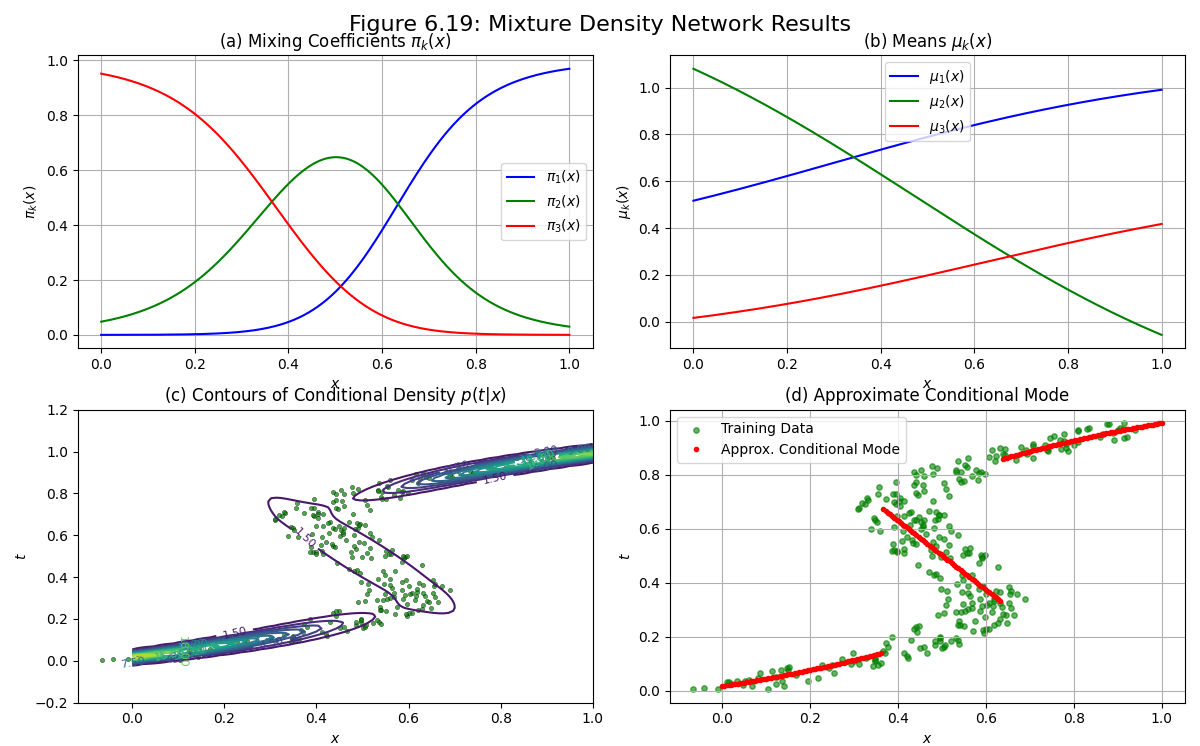
\includegraphics[height=0.7\textheight]{fig619_result.png}
        \caption{(a)分量配置、(b)分量的均值、(c)条件概率密度、(d)近似条件众数}
    \end{figure}
\end{frame}


% 第十部分：应用
\section{应用}
\begin{frame}
    \frametitle{10. 混合密度网络的应用}
    \begin{itemize}
        \item \textbf{逆问题}：机器人控制、计算机视觉（姿态估计）。
        \item \textbf{序列建模}：手写合成（Graves, 2013）、语音生成。
        \item \textbf{不确定性量化}：不仅预测一个值，还预测反映置信度的分布。
        \item \textbf{物理/科学}：建模复杂的物理关系（例如，系外行星表征）。
        \item \textbf{生成任务}：提供一种可学习的、参数化的复杂输出分布建模方法。
    \end{itemize}
\end{frame}

% 第十一部分：优势
\section{优点与缺点}
\begin{frame}
    \frametitle{11. 混合密度网络的优点}
    \begin{itemize}
        \item 能够建模\alert{复杂、多峰的条件分布}。
        \item 提供预测中的\alert{不确定性}度量。
        \item 灵活的框架：可以调整分量数量 $ K $ 和网络架构。
        \item 统一了函数逼近和密度建模。
        \item 输出混合模型的可解释参数。
    \end{itemize}
\end{frame}

% 第十二部分：缺点
\begin{frame}
    \frametitle{12. 混合密度网络的缺点}
    \begin{itemize}
        \item 比标准回归/分类网络更复杂。
        \item 需要更多参数（特别是当 $ K $ 或 $ L $ 较大时）。
        \item 训练可能更具挑战性（例如，模式坍塌、梯度消失）。
        \item 选择分量数量 $ K $ 需要调优。
        \item 假设组件为高斯分布（尽管可以使用其他类型的组件）。
    \end{itemize}
\end{frame}

% 第十三部分：总结
\section{总结}
\begin{frame}
    \frametitle{13. 总结}
    \begin{itemize}
        \item 混合密度网络（MDN）是一种用于建模复杂条件概率分布 $ p(\mathbf{t} | \mathbf{x}) $ 的强大工具。
        \item 它将神经网络与高斯混合模型（GMM）相结合。
        \item 网络输出 GMM 的参数（混合系数、均值、方差）。
        \item 这对于具有多峰输出的问题特别有用（逆问题）。
        \item 通过最大似然（负对数似然损失）进行训练。
        \item 提供超越单一预测点的丰富预测，包括不确定性信息。
    \end{itemize}
\end{frame}

% 第十四部分：参考资料
\begin{frame}
    \frametitle{14. 参考文献}
    \begin{itemize}
        \item 教材：Bishop, C. M. \& Bishop, H. (2023). Deep Learning Foundations and Concepts. Springer Nature Switzerland AG. 
        \item Bishop, C. M. (1994). Mixture Density Networks. Technical Report NCRG/94/004, Aston University.
        \item Graves, A. (2013). Generating Sequences With Recurrent Neural Networks. arXiv preprint arXiv:1308.0850.
        \item 博客文章: blog.otoro.net (使用TensorFlow的混合密度网络)。
        % 根据需要添加更多参考文献
    \end{itemize}
\end{frame}

\begin{frame}
    \frametitle{15. 课程网站资源}
    \begin{center}
    \url{https://gitee.com/liqing-wang-cscs/deep-learning-foundations} 
    \end{center}

    % 课程网站包含内容：
    \begin{itemize}
        \item 课文解读
        \item 例子代码
        \item 本幻灯片
        \item 课文相关练习题
    \end{itemize}
\end{frame}

\end{document}